% Introduction to what a Packet storage is. Discuss its strcuture.
% Where is it used, and how is it useful.
% How many controllers it has (and why)
% What is in the report (section-wise)

The project described in this report is based on the modelling and verification of a packet storage system. The packet storage system is inspired by the distributed controller of an operational product manufactured by Vanderlande, a Dutch company. 
The aim of this project is to model the system such that it uses $5$ controllers, which can communicate with each other, $2$ elevator platforms, one rack where packets could be stored and a conveyor each for accepting and delivering packets.

The figure \ref{fig:packet_storage} below shows the high level view of such a system.
\begin{figure}[h]
\center
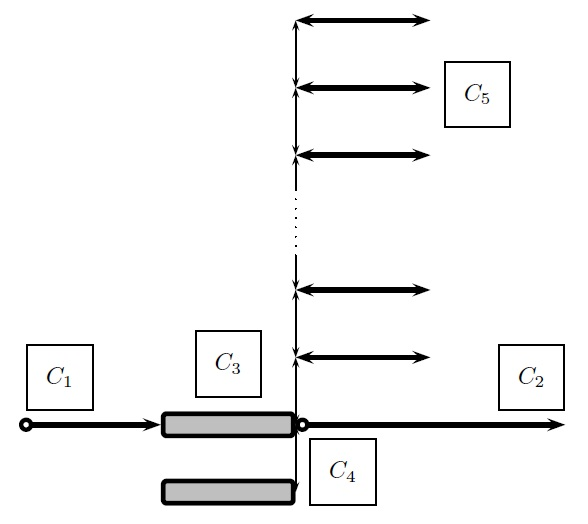
\includegraphics[width=0.6\textwidth]{packet_storage_diag}
\caption{Packet storage system, courtesy \cite{problem_statement}}
\label{fig:packet_storage}
\end{figure}

Our motivation in this project is to model these $5$ controllers with their interactions, describe their behaviour using mCRL2 language and then to perform verification using mCRL2 toolset to prove that all the requirements of the system are met.

The next section in the report describes the \textit{system details and design decisions}. In the subsequent section, the \textit{global requirements} for such a system chosen are listed out in brief, along with high level \textit{architecture} of the system. 

Further sections describe the external interactions in the system, translated requirements, discussion on controllers with its labelled transition diagram(LTS). In the end, verification of these requirements is done using modal calculus and verification tools as part of mCRL2 tool set. The verification is done to assert that the stated requirements are same as what system can achieve, and does not deviate from the actual model design.